% 插入位置：文本小节中“最终得到 X^{(T)}...同时保留...映射。”这一段之后，声学小节之前。
% 将 figures/fig_5_3_text_mapping.pdf 放入论文工程的 figures 目录；需要 graphicx 宏包。
图~\ref{fig:p1_text_mapping}以原词\texttt{adhesives}为例，展示子词表示向词级表示的聚合过程。该词在原文中的字符区间为$[21,30)$，经WordPiece划分为\texttt{ad}、\texttt{\#\#hesive}和\texttt{\#\#s}，对应区间分别为$[21,23)$、$[23,29)$和$[29,30)$。完整转写参与上下文编码后，取这三个子词的最后一层隐藏向量进行平均，得到该词对应的768维文本表示。

\begin{figure}[htbp]
    \centering
    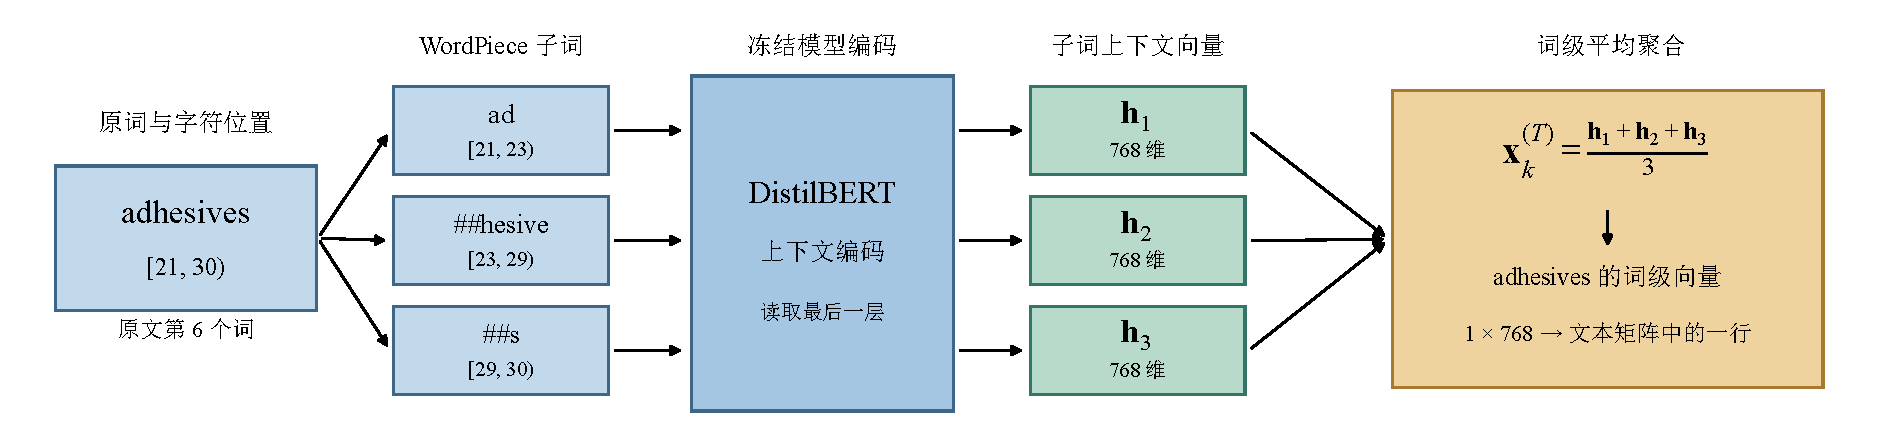
\includegraphics[width=\linewidth]{figures/fig_5_3_text_mapping.pdf}
    \caption{基于字符位置的子词映射与词级语义表示构建。示例来自样本\texttt{-3g5yACwYnA\$\_\$3}，字符位置从0开始，区间左闭右开；图中$\boldsymbol h_1$、$\boldsymbol h_2$和$\boldsymbol h_3$仅为所展示子词的局部编号，向量用符号表示。}
    \label{fig:p1_text_mapping}
\end{figure}
